\section{Methods}\label{sec:pecanrtm-methods}

\subsection{Inversion procedure}

The PROSPECT 5 model simulates the full spectral reflectance and transmittance of a leaf over the 400--2500 nm range using five key parameters related to leaf structure and biochemistry~\cite{feret_2008_prospect}.
In the PROSPECT model, a leaf is treated as a set of N partially transparent flat plates, each with wavelength-dependent transmissivity $k\lambda$.
Transmissivity $k\lambda$ is based on the linear combination of empirically calibrated specific absorption spectra for total chlorophyll (a and b), total carotenoids, water, and dry matter (e.g.\ cellulose, lignin, protein) multiplied by their respective quantities (given by the parameter values: Cab, Car, Cw, Cm) (Table~\ref{tab:pecanrtm-parameters}; Figure S1). %TODO: Figure reference

\begin{table}
  \caption{%
    Summary of PROSPECT 5 parameters.
    Ranges for Car, Cw, and Cm are based on the datasets used for their calibration (ANGERS for Cab and Car, LOPEX for Cw and Cm) as reported in Feret et al.~(2008).
    The ranges for N and Cab are calculated from the LOPEX and ANGERS databases, respectively.
    Units for Cw and Cm are adjusted for readability (original units are $g cm^{−2}$).
  }\label{tab:pecanrtm-parameters}
  \resizebox{\textwidth}{!}{%
    \begin{tabular}{cccc}
      \toprule
      Parameter & Description & Unit & Range \\
      \midrule
      N & Structural parameter; effective number of mesophyll layers & Unitless & 1.09 to 3.00 \\
      Cab & Total chlorophyll (a and b) density & μg cm−2 & 0.78 to 106.72 \\
      Car & Total carotenoid density & μg cm−2 & 0 to 25.3 \\
      Cw & Equivalent water thickness & g m−2 & 43 to 439 \\
      Cm & Leaf dry matter content per unit area & g m−2 & 17 to 152 \\
      \bottomrule
    \end{tabular}
  }
\end{table}

The objective of RTM spectral inversion is to estimate the physical RTM parameters from the observed spectral information.
This is accomplished through a statistical inversion, wherein we seek the set of parameters that minimizes the residual error between PROSPECT-modeled and measured reflectance.
Our approach to the inversion of PROSPECT is distinct from previous studies~\cite{combal_2003_retrieval,feret_2008_prospect,feret_2011_optimizing,li_2011_retrieval,li_2013_retrieval} in two important ways.
First, whereas many past studies use both reflectance and transmittance to estimate parameters, we use only reflectance.
Reflectance is generally easier to measure than transmittance, which requires special instrumentation such as integrating spheres that often have inadequate designs and yield poor signal-to-noise ratios, especially in the longer wavelengths (i.e.\ $> 2 \mu \texttt{m}$).
As well, inversion on reflectance data alone allows transmittance measurements as optional data for independent validation.
Second, unlike past leaf-level PROSPECT inversion studies that only provide point estimates of parameters, we performed our analysis within a Bayesian framework that provides the joint probability distribution of the PROSPECT 5 parameters, $\theta = {N, Cab, Car, Cw, Cm}$, and the residual standard deviation, $\sigma$, as the output.
The general mathematical statement of this posterior distribution is given as follows:

\[ P(\theta, \sigma \mid X) \sim P(X \mid \theta, \sigma)P(\theta)P(\sigma) \]
\[ P(X \mid \theta, \sigma)\ \sim Normal(PROSPECT5(\theta) \mid X, \sigma) \]

where $PROSPECT5(\theta)$ is the modeled reflectance given $\theta$, and $X$ is a vector of observed reflectance values.
The residual error is assumed to be normally distributed with a mean of 0 and standard deviation of $\sigma$.

We set the prior distribution for N to a lognormal distribution shifted to have a minimum of 1, and parameterized based on a review of literature using the PROSPECT model~\cite{lemaire_2004_towards,ferreira_2013_analyzing,croft_2014_applicability} (Figure S2). %TODO: Figure reference
We assigned the remaining parameters log-normal priors based on summary statistics and histograms from the LOPEX, ANGERS, HAWAII, and CALMIT spectral databases as reported by Feret et al.~(2008) \nocite{feret_2008_prospect} (Figure S2). %TODO: Figure reference
The residual standard deviation $\sigma$ was assigned an uninformative inverse gamma prior, which is conjugate with the normal distribution and therefore allows for computationally efficient Gibbs sampling.

We sampled the joint posterior distribution of the PROSPECT 5 parameters using the Metropolis-Hastings (MH) algorithm with adaptive block sampling~\cite{haario_2001_adaptive}.
For this, we initialized each inversion using parameter values drawn at random from the prior distributions.
For each inversion, we ran the algorithm five times (i.e.\ five independent chains) for 100,000 iterations each.
At each iteration, the algorithm proposes a parameter vector, calculates the vector’s likelihood based on the observations and the prior, and accepts or rejects the vector based on this likelihood.
The proposal step performs a random draw from a multivariate normal distribution centered on the last accepted parameter vector.
The covariance matrix for the multivariate normal proposal distribution was re-computed every 100 iterations as follows:
(1) the univariate standard deviation of each parameter and the Pearson product-moment correlation matrix were computed;
(2) the standard deviation vector was multiplied by the ratio of the acceptance rate in the last 100 samples to the target acceptance rate (set to 0.234, as per Haario et al. 2001);
(3) the resulting standard deviation vector was converted to a diagonal matrix and multiplied to both sides of the correlation matrix to give a re-scaled covariance matrix. 
For each inversion, we determined MCMC convergence based on a value of the Gelman-Rubin multivariate potential scale reduction factor of less than 1.1 (Gelman \& Rubin 1992, as implemented in the R \texttt{coda} package v.0.18--1 by Plummer et al.). \nocite{gelman_1992_inference,r_coda}
For runs that did not converge, we repeated this process with a 20\% smaller target acceptance rate for the adaptation step, which increases the size of the sampling space for each chain and therefore reduces the likelihood of getting trapped in local minima. 
Across the >10,000 inversions performed in this study, only five failed to converge (after five inversion attempts)—all for simulated CHRIS-Proba spectra (see Section 2.3)—and we excluded these data points from our analysis. %TODO: Section reference
We visually examined a random subset of the resulting trace plots and autocorrelograms and determined that a common burn-in period of 80,000 samples and a thinning interval of 20 was sufficient for an accurate and representative sample of the joint posterior distribution.
After applying the burn-in and thinning filter, we calculated the mean, standard deviation, and 95\% confidence intervals of the sampled parameter values (Figure S3). %TODO: Figure reference

With chains running in parallel, the inversion of one leaf spectrum with our specifications takes approximately 4 minutes (on one Intel Xeon X5570 CPU @ 2.93GHz), and running the entire set of over 10,000 inversions required for this paper took several days (running up to 16 inversions simultaneously on a high performance computing cluster).
That being said, we anticipate that recoding of the algorithm from R to a compiled language will dramatically increase (>50x) the computational efficiency of our approach.

The inversion algorithm described above is available as an open-source, publicly-available R~\cite{rstats} package housed within the PEcAn ecoinformatics toolbox \texttt{github.com/pecanproject/pecan/tree/master/modules/rtm}~\cite{dietze_improving_2013,lebauer_facilitating_2013}.
This package allows users to simulate spectra using the PROSPECT family of radiative transfer models and apply our inversion algorithm to their own models and data.
For more information, refer to the package vignette on the PEcAn tutorials page \texttt{pecanproject.github.io/tutorials.html}.

\subsection{Validation}

\subsubsection{Data}

We tested the ability of our inversion to accurately estimate leaf traits using data collected as part of the NASA Forest Functional Types (FFT) campaign~\cite{deel_2012_relationship,serbin_spectroscopic_2014,singh_imaging_2015}.
This dataset consists of leaves collected from various positions within the canopy for 52 species from 13 sites across the Northeast and Midwest USA\@.
An Analytical Spectral Devices (ASD) FieldSpec 3 Full Range (350 to 2500 nm) Spectroradiometer was used together with a leaf clip and internal calibrated light source to measure reflectance on the adaxial surface of 1348 unique leaves.
For a subset of 765 of these leaves, the same instrument was used with an ASD integrating sphere setup to measure transmittance through the leaf adaxial surface.
Our database included both broadleaf and conifer species.
For conifer measurements, we constructed edge-to-edge mats of needles larger than the spot size of the light source~\cite{serbin_2012_spectroscopic,singh_imaging_2015}.
As detailed in Serbin (2012), we found minimal changes in reflectance/transmittance measurement up to a threshold of differing gaps between needles. \nocite{serbin_2012_spectroscopic}
These observations are henceforth referred to as “FFT measured reflectance and transmittance,” respectively.
In addition to spectral measurements, laboratory measurements of leaf dry mass per unit area (LMA) and equivalent water thickness (EWT) were available for 950 leaves.
For further information on the sampling methodology, see Serbin et al.~(2014). \nocite{serbin_spectroscopic_2014}

During exploratory analysis, we observed that inversion results by leaf habit displayed some distinct differences and conifer species were consistently less accurate than results for broadleaved species, reflecting ecological differences in leaf structure that are not well represented by the PROSPECT model.
Therefore, to better contextualize our results, we performed both validation steps for the entire data set and separately for broadleaved and conifer species.
However, even within the conifer functional type, we found certain species and foliar morphologies showed much larger errors than others.
These differences could be ecological in nature or an artifact related to the challenges of measuring full-range reflectance and transmittance of different types of conifer needles. 
To investigate whether these errors aligned with established ecological classifications, we grouped species based on their approximate succession (``early'', ``mid'', or ``late''), following the general classification scheme of Dietze \& Moorcroft (2011), \nocite{dietze_2011_tree}
except that we grouped the ``Northern'' and ``Southern Pine'' functional types as ``early conifer.''
Classification based on succession is useful for this study because it is indicative of plant shade tolerance~\cite{dietze_2011_tree}, which is closely linked to leaf structure and biochemistry~\cite{poorter_2009_causes}.

We applied our inversion algorithm individually to each of the FFT measured reflectance spectra ($n = 1348$), resulting in an estimate of the joint probability distribution of the PROSPECT 5 parameters for each leaf.
We then generated a dataset of synthetic reflectance spectra (“FFT simulated reflectance”) by using the middle 90\% of these parameter estimates ($n = 1040$) as inputs to the PROSPECT 5 model.
These synthetic reflectance spectra were used as data in the sensor simulation experiment (Section 2.3). %TODO: Section reference
We used real parameter estimates rather than random draws from a distribution to preserve their ecological ranges and covariances resulting from within- and between-species tradeoffs in traits such as those described for the leaf economics spectrum~\cite{wright_worldwide_2004}. 

We then performed two different tests to evaluate the accuracy of these parameter estimates:
(1) We compared the FFT simulated reflectance and transmittance to measured reflectance and transmittance, and
(2) we directly compared the inversion estimates of PROSPECT 5 parameters Cw and Cm to measured values of EWT and LMA, respectively.

\subsubsection{Reflectance and transmittance}

A common way to validate model inversion is to run the model in forward mode using the estimated parameters as inputs and compare the output to the original data.
For our study, we used the inversion estimates of the PROSPECT parameters as inputs to the PROSPECT model to predict reflectance and transmittance spectra, which we then compared to the observed reflectance and transmittance.
Errors in spectral inversion can originate from multiple sources, including measurement error (both trait and spectra), failure of the PROSPECT model to fully capture leaf spectral features (i.e.\ model formulation error), and parameter identifiability issues in the inversion algorithm.
To isolate algorithmic error, we first performed the validation on a set of synthetic reflectance and transmittance spectra ($n = 1348$).
To investigate the remaining sources of error, we performed the same validation on FFT measured reflectance ($n = 1348$) and transmittance ($n = 765$) spectra.
For both reflectance and transmittance, we calculated the mean and 90\% and 95\% confidence intervals on the absolute error ($\text{simulated} - \text{measured}$) at each wavelength.
The overlap of the 95\% confidence interval with 0 was used to judge statistical significance.
To facilitate comparison with other RTM inversion studies~\cite{feret_2008_prospect,divittorio_2009_enhancing}, we also computed the root mean square error (RMSE), bias (BIAS), and bias-corrected RMSE (SEPC) averaged across the visible (VIS, 400--800 nm) and near-infrared (NIR, 801--2500 nm) regions of the spectrum:

\[ RMSE = \sqrt{\frac{\sum{{(x_i - x_0)}^2}}{n}} \]
\[ BIAS = \frac{\sum{x_i - x_0}}{n} \]
\[ SEPC = \frac{\sum{{(x_i - x_0 - BIAS)}^2}}{n} \]

where $x_i$ is the simulated value (reflectance or transmittance), $x_0$ is the observed value, and $n$ is the number of spectra considered.

\subsubsection{Leaf water content and mass per area}

For leaves that had paired measurements of reflectance and EWT and LMA ($n = 950$), we compared the mean inversion estimates for PROSPECT parameters Cw and Cm to measured values of EWT and LMA, respectively.
For each, we compared the mean inversion estimate to the measured value via the RMSE, BIAS, and SEPC as above (with inversion estimate x and measurement xo) as well as relative RMSE (RMS\%E) and the relative bias-corrected RMSE (CV):

\[ RMS\%E = \sqrt{\frac{\sum{{\left(\frac{x_i - x_0}{x_0} \right)}^2}}{n}} \times 100\% \]
\[ CV = \frac{SEPC}{x_0} \times 100\% \]

\subsection{Sensor simulation experiment}

\begin{table}
  \caption{%
    Spectral, spatial, and temporal characteristics of remote sensing platforms and instruments considered in the sensor simulation experiment.
    Note that AVIRIS spatial resolution is dependent on aircraft altitude and instrument field of view.
  }\label{tab:pecanrtm-sensors}
  \resizebox{\textwidth}{!}{%
    \begin{tabular}{cccccc}
      \toprule
      Sensor & Number of Bands & Spectral range (nm) & Bandwidth (nm) & Spatial resolution (m) & Revisit time (days) \\
      \midrule
      AVIRIS NG & 416 & 380 to 2510 & 5 & 0.3 to 4.0 & On-demand \\
      AVIRIS Classic & 216 & 400 to 2500 & 10 & $<10$ to 20 & On-demand \\
      CHRIS-Proba & 62 & 410 to 1050 & 1.5 to 12 & 36 & 7 to 8 \\
      Hyperion & 225 & 350 to 2500 & 10 & 30 & 16 \\
      Landsat 5 (TM) & 6 & 450 to 2350 & 60 to 270 & 30 & 16 \\
      Landsat 7 (ETM+) & 6 & 440 to 2350 & 60 to 280 & 30 & 16 \\
      Landsat 8 (OLI) & 8 & 435 to 2295 & 20 to 185 & 30 & 16 \\
      MODIS & 7 & 459 to 2155 & 20 to 50 & 250 to 500 & 1 to 2 \\
      VIIRS & 10 & 402 to 2275 & 15 to 60 & 750 & 1 to 2 \\
      AVHRR & 3 & 580 to 1640 & 100 to 275 & 1090 & 1 \\
      \bottomrule
    \end{tabular}
  }
\end{table}

Recent work has shown that PLSR estimates of foliar nitrogen content are less sensitive to spectral resolution than to other factors such as spatial resolution and sensor fidelity~\cite{lepine_2016_examining}.
However, the PLSR approach implemented in that study was unable to quantify the uncertainty around the nitrogen estimates.
We hypothesize that the spectral characteristics of most common remote sensing platforms are sufficient to accurately estimate the leaf biophysical parameters modeled by PROSPECT, but that the uncertainties in these parameters will increase with declining spectral resolution.
To test this hypothesis, we transformed the FFT simulated reflectance spectra using the relative spectral response functions of 11 common remote sensing platforms (Table~\ref{tab:pecanrtm-sensors}, Figure S4), %TODO: Figure reference
and used our Bayesian inversion of PROSPECT 5 to retrieve the starting parameters from the transformed spectra.
For input parameters, we used the inversion results from measured spectra, thereby capturing a large range of ecologically realistic values and preserving inherent covariances between parameters.
To account for observation error, we simulated Gaussian random noise (with mean 0 and standard deviation $2.5 \times 10^{-4}$) smoothed with a Gaussian filter (kernel width 11) to account for inherent autocorrelation in hyperspectral measurements (Figure S5). %TODO: Figure reference

We then examined how two characteristics of the inversions varied between sensors:
Relative bias ($\alpha$) indicates how closely the mean parameter estimate ($\mu$) matched the true value ($p$) and is a useful measure for describing the accuracy of the estimate’s central tendency.

\[ \alpha = \frac{\mu - p}{p} \]

Uncertainty ($\pi$) describes the width of the 95\% confidence interval of the estimate ($s$) relative to the mean value,
and is useful for ascertaining the precision with which the inversion is able to estimate a parameter.

\[ \pi = \frac{s}{\mu} \]

We note that both statistics are normalized to facilitate inter-parameter comparison.
Both metrics were computed for each parameter for each inversion and then averaged over all simulated spectra.

We recognize that this experiment does not fully capture all of the variability associated with inversion of real observations from these sensor systems given its failure to account for canopy structure, atmospheric effects, sun-sensor geometry, and sensor radiometric resolution.
However, this experiment is capable of illustrating the ability to characterize uncertainty in inversion results and improves the confidence with which we can extract information from lower quality data sources.
Moreover, this experiment sets a theoretical limit on the accuracy and precision of leaf trait retrieval from spectral RTM inversion, thereby contextualizing past RTM inversion results~\cite{zhang_2005_estimating,zhang_2006_characterization,zhang_2009_satellite,zhang_2012_estimating} and guiding future research in the field.

The entire workflow for this paper is summarized in Figure 1. %TODO: Figure reference
The data and R source code for performing all analyses in this study have been made publicly available at \texttt{github.com/ashiklom/sensor-manuscript}.

\begin{figure}
  \centering
  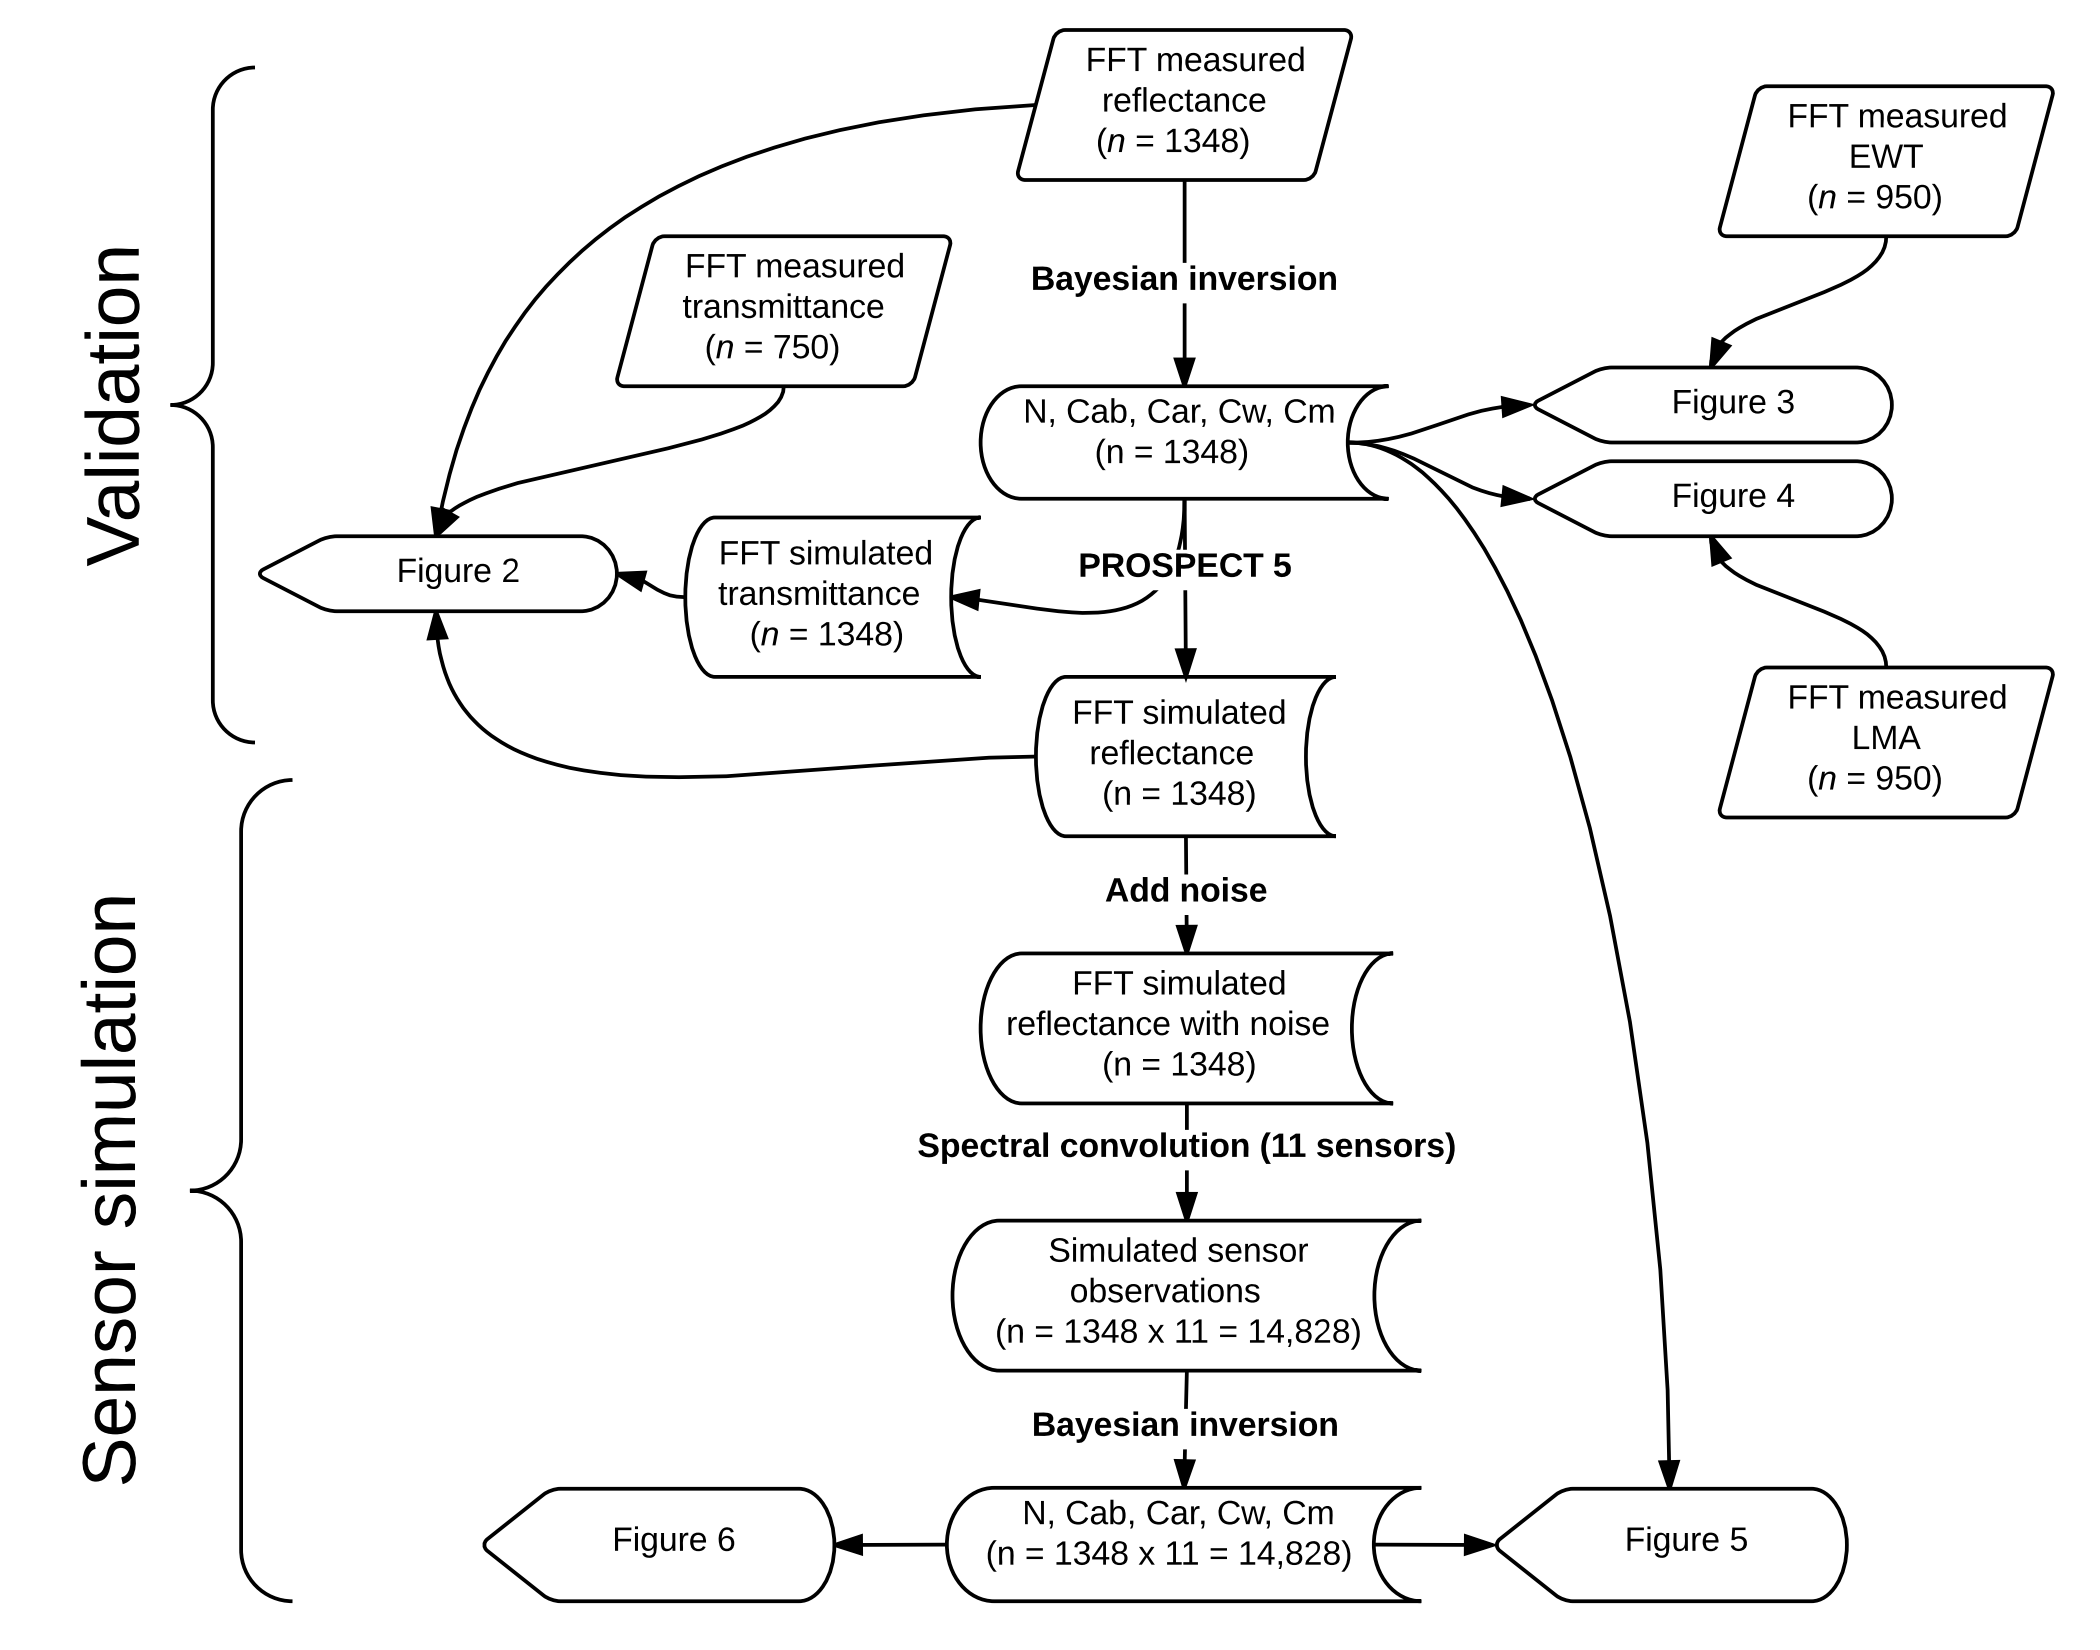
\includegraphics[width=\textwidth]{2_rtm_inversion/figures/workflow.png}
  \caption{%
    Workflow illustrating the steps in this study as well as the figures to which they correspond.
  }\label{fig:pecanrtm-workflow}
\end{figure}
